\documentclass{article}
\usepackage[utf8]{inputenc}
% \usepackage{newunicodechar}
% \newunicodechar{fi}{fi}
% \newunicodechar{ff}{ff}
\usepackage{amsmath}
\usepackage{mathtools}
\usepackage{booktabs}
\usepackage{enumerate}
\usepackage{extarrows} % extra arrows
\usepackage{graphicx}                 % 图形
\usepackage{tikz} % draw graph in latex
\usetikzlibrary{decorations.pathreplacing} % decoration package for tikz
\graphicspath{{figures/}}        % 图片文件路径
\newlength\imagewidth
\newcommand{\myref}[1]{Equation \eqref{#1}}
\setlength\imagewidth{0.45\columnwidth}

% \pagestyle{empty}
% \newlength{\defwidth}
% \textwidth = 17.5cm
% \defwidth  = 15.0cm
% \textheight = 26cm
% \topmargin = -2.0cm
% \oddsidemargin = -0.5cm
% \evensidemargin = 0.25cm
% \parindent 0mm
% \sloppy
% \setlength{\parskip}{2mm plus1mm minus1mm}

\title{Pollution Control 2}
\author{Zhao Chi, Wu Haitao}
\date{\today}


\begin{document}
    \maketitle
\section*{Question}

\begin{figure}[ht]
    \centering
    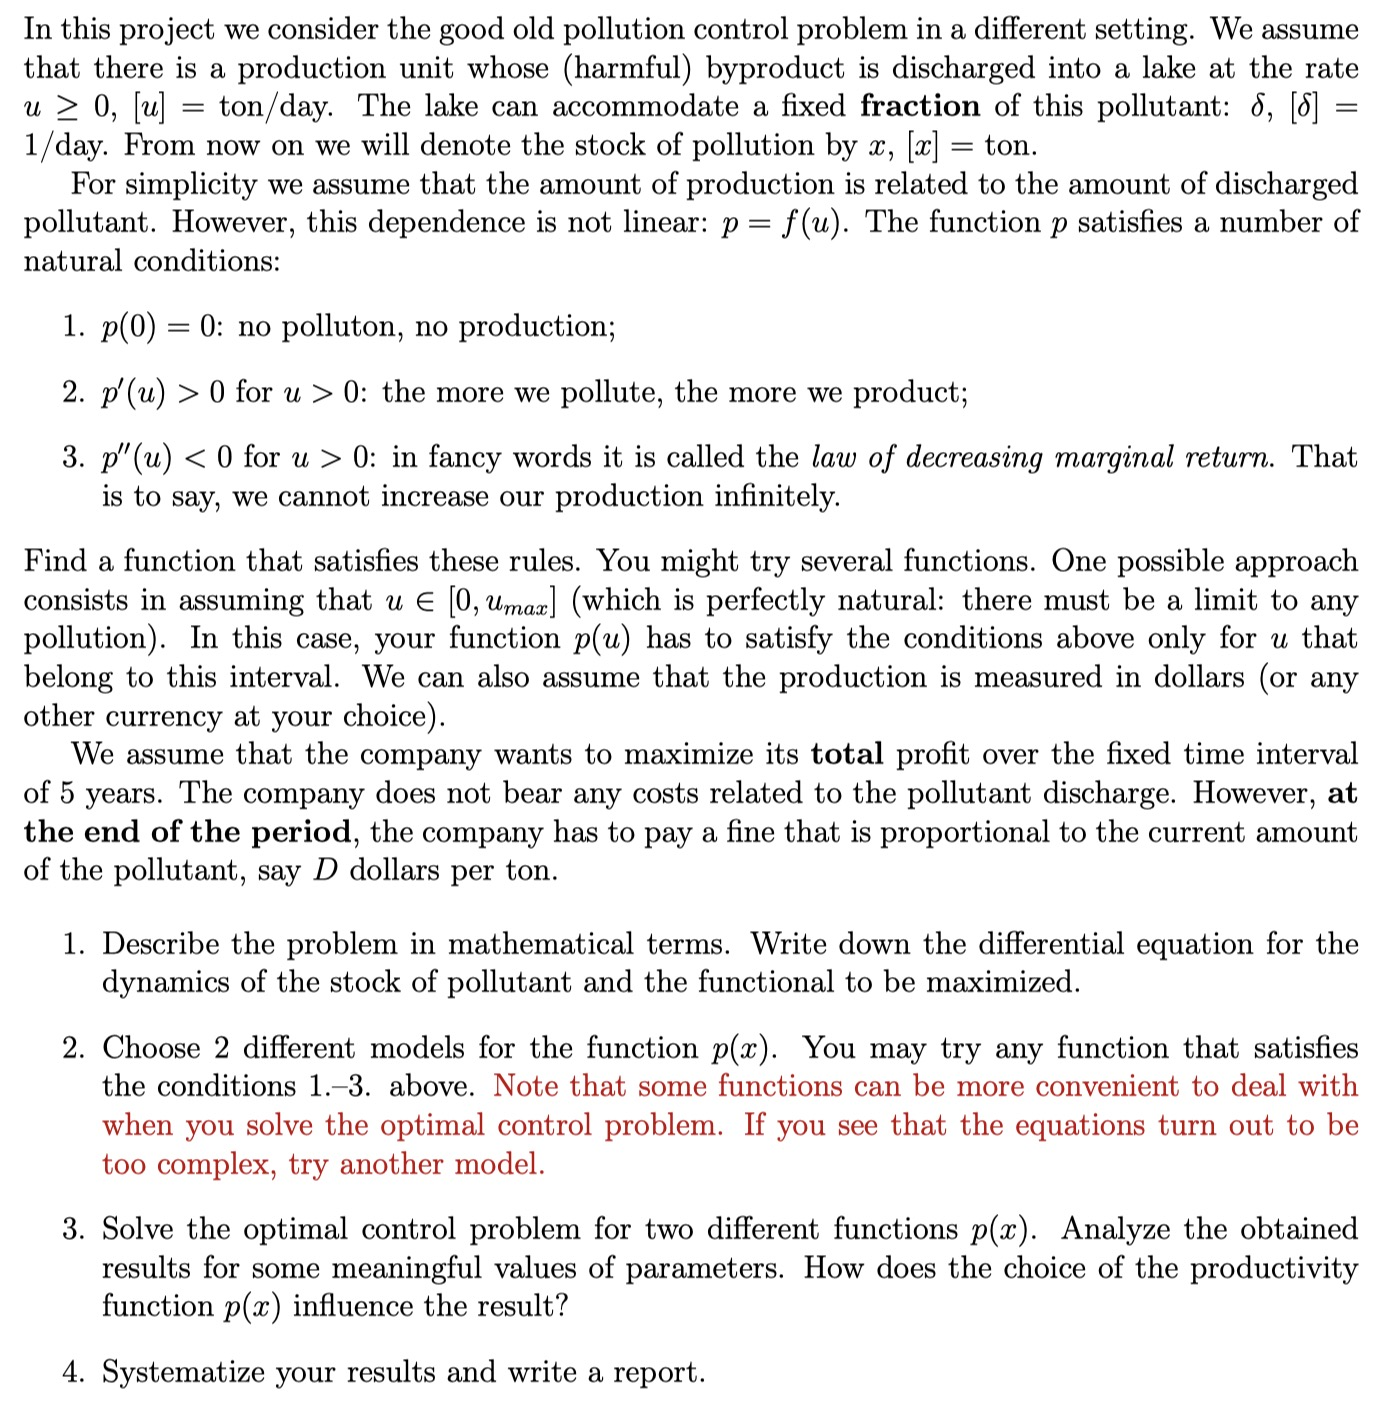
\includegraphics[width=2.2\imagewidth]{Question.png}
    % \caption{Question}
    %   \label{fig:q}
\end{figure}


\section*{Solution}

{\bf Question 1:} Describe the problem in mathematical terms. Write down the differential equation for the dynamics of the pollutant and the functional to be maximized.

From the Question description, it's not hard to find that as the time change, the total amount of pollution increases $u$ per unit time. Besides, consider the absorption of pollutants by the lake itself. Therefore we can write down the relationship in differential equation form.

\begin{equation}\label{cd:initial_condition}
    \dot{x}=u-\delta x, x(0)=x_0\ \text{and}\ {\color{red} x(T)=x_T\ \text{only be used for fixed endpoint}}
\end{equation}

There are many function $p(u)$ satisfy the following natural conditions:

\begin{enumerate}
    \item $p(0)=0$;
    \item $p'(u)>0\ \text{for}\ u\in(0,u_{max}]$;
    \item $p''(u)<0\ \text{for}\ u\in(0,u_{max}]$.
\end{enumerate}

$p(u)$ is the amount of production, assume the profit is $a\ \text{dollars/unit}$. Therefore, the instantaneous payoff function is defined as:

\begin{equation}\label{eq:payoff_funtion_instant}
    f_0(u)=ap(u)
\end{equation}

The company want to maximize it's \textbf{total} profit over the fixed time interval of 5 years and the company does not bear any costs related to the pollutant discharge. However, at \textbf{the end of the period}, the company has to pay a fine that is proportional to the current amount of the pollutant, say $D$ dollars per ton. Therefore we have a terminal cost.

\begin{equation}\label{eq:terminal_cost}
    F_0(x(T))=Dx(T)
\end{equation}

If \textbf{endpoint} is \textbf{fixed}, then Equation \eqref{eq:terminal_cost} is a constant. It doesn't influence out optimization problem. And $a$ is a constant, hence maximize Function \eqref{eq:payoff_funtion_instant} is equivalent to maximize Function $p(u)$.

% It doesn't influence our optimization problem.


The total payoff function to be maximized  is:

\begin{equation}\label{eq:optfunction_without_terminal_cost}
    J(u,T)=\int_{0}^{T}p(u)dt\rightarrow \max_{u}
\end{equation}

To simplisfy the calculation, in the following I use $D(0,1]$ instead of $\frac{D}{a}$. \footnote{In deed, the fundamental operation of the optimized equation and constant does not affect the value of the solution. The original expression $\frac{D}{a}\leq 1$, which means the penalty in the terminal time doesn't large than profit per/ton.} 

If \textbf{endpoint} is \textbf{free}, then the total payoff function to be maximized is:

\begin{equation}\label{eq:optfunction_with_terminal_cost}
    J(u,T)=\int_{0}^{T}p(u)dt-Dx(T)\rightarrow \max_{u} 
\end{equation}

\noindent{\bf Question 2:} Choose 2 different models for the function $p(u)$ that satisfies the conditions 1.-3. above.

Assume, $u_{max}=b$, the following two models satisfy conditions 1-3.

\begin{gather}
    \begin{aligned}
        \textbf{Model 1: } & p(u)=-\frac{1}{2}u^2+bu\\
        \textbf{Model 2: } & p(u)=\ln (u+1) 
    \end{aligned}
\end{gather}

\noindent{\bf Question 3:} Solve the optimal control problem for two different functions $p(u)$. Analyze the obtained results for some meaningful values of parameters. How does the choice of the productivity function $p(u)$ influence the results.

Don't consider leap years, in this case, $T=5\times 365=1825.$

{\bf Model 1-1(no terminal cost)::} Our optimization problem is:
\begin{equation}
    J(u,T)=\int_{0}^{T}\bigl(-\frac{1}{2}u^2+bu\bigr)dt\rightarrow \max_{u}\ s.t. \eqref{cd:initial_condition}
\end{equation}
\begin{enumerate}[a)]
    \item Write down the Hamiltonian Function:
            \begin{equation}\label{eq:hamiltonian}
                H(x,u,\psi)=-\frac{1}{2}u^2+bu+\psi (u-\delta x)
            \end{equation}
    \item It's first order partial derivatives w.r.t $u$ is:
            \begin{equation}
                \frac{\partial }{\partial u}H(x,u,\psi)=-u+b+\psi
            \end{equation}
             According to the first order extremality condition:
             \begin{equation}\label{eq:optc_with_psi}
                u^*(t)=b+\psi(t)
             \end{equation}
             And $\frac{\partial^2 }{\partial u^2}H(x,u,\psi)\big|_{u=u^*}<0$, we can conclude that the Hamiltonian $H$ is concave w.r.t $u$.
    \item We substituete \eqref{eq:optc_with_psi} into \eqref{eq:hamiltonian} to get the maximal Hamiltonian Function:
             \begin{equation}
                \mathcal{H}(x, \psi)=H(x,u^*,\psi)=\frac{1}{2}(b+\psi)^2-\delta\psi x
             \end{equation}
    \item The canonical form is writen as:
             \begin{equation}\label{eq:canonical_form}
                 \begin{dcases}
                    \dot{x}= \frac{\partial }{\partial \psi}H(x,u,\psi)\bigg|_{u=u^*}=b+\psi(t)-\delta x\\
                    \dot{\psi}=-\frac{\partial }{\partial x}H(x,u,\psi)\bigg|_{u=u^*}=\delta\psi(t)
                \end{dcases}
             \end{equation}
    \item From D.E.S \eqref{eq:canonical_form}, it's not hard to find:
             \begin{equation}\label{eq:psi_with_psi0}
                 \psi(t)=\psi_0 e^{\delta t}
             \end{equation}
    \item According to D.E.S \eqref{eq:canonical_form} and Equation \eqref{eq:psi_with_psi0}, we can find the optimal trajectory:
             \begin{equation}\label{eq:optx_with_psi0}
                 x^*(t)=x_0e^{-\delta t}+\frac{b}{\delta}(1-e^{-\delta t})+\frac{\psi_0}{2\delta}(e^{\delta t}-e^{-\delta t})
             \end{equation}
    \item From Equation \eqref{eq:optx_with_psi0} and initial condition $x(T)=x_T$, we can find:
             \begin{equation}
                 \psi_0=\frac{2\delta}{e^{\delta T}-e^{-\delta T}}\biggl[x_T-x_0e^{-\delta T}-\frac{b}{\delta}(1-e^{-\delta T})\biggr] \label{eq:psi0}
             \end{equation}
            Then:
            \begin{equation}\label{eq:psi}
                \psi(t)=\frac{2\delta e^{\delta t}}{e^{\delta T}-e^{-\delta T}}\biggl[x_T-x_0e^{-\delta T}-\frac{b}{\delta}(1-e^{-\delta T})\biggr]
            \end{equation}
    \item    Substitute $\psi(t)$ into Equation \eqref{eq:optc_with_psi}, we can find the optimal control:
        \begin{equation}\label{eq:optc}
            u^*(t)=b+\frac{2\delta e^{\delta t}}{e^{\delta T}-e^{-\delta T}}\biggl[x_T-x_0e^{-\delta T}-\frac{b}{\delta}(1-e^{-\delta T})\biggr]
        \end{equation}
        Since $u^*(t)\in [0,b]$, we need to keep $\biggl[x_T-x_0e^{-\delta T}-\frac{b}{\delta}(1-e^{-\delta T})\biggr]<0$
    \item Substitute $\psi_0$ into Equation \eqref{eq:optx_with_psi0}, we can find the optimal trajectory:
        \begin{equation}\label{eq:optx}
            x^*(t)=x_0e^{-\delta t}+\frac{b}{\delta}(1-e^{-\delta t})+\frac{e^{\delta t}-e^{-\delta t}}{e^{\delta T}-e^{-\delta T}}\biggl[x_T-x_0e^{-\delta T}-\frac{b}{\delta}(1-e^{-\delta T})\biggr]
        \end{equation}
        % Since the total pollution can not be negative, we need assure $x(t)\geq 0\ \text{for}\ t\in[0,T]$. From the Equation \eqref{eq:optx}, we can find that $t^*$ satisfies $x(t)\geq 0$ for $t\in [0,t^*]$. Therefore for $t\in [0,t^*]$, $x^*(t)$ would following the Equation \eqref{eq:optx} and for $t\in [t^*,T]$, $x^*(t)=u^*(t)-\delta x$.
\end{enumerate}

{\bf Model 1-2(terminal cost):} Our optimization problem is:
\begin{equation}
    J(u,T)=\int_{0}^{T}\bigl(-\frac{1}{2}u^2+bu\bigr)dt-Dx(T)\rightarrow \max_{u}\ s.t. \eqref{cd:initial_condition}
\end{equation}

Same procedure as \textbf{Model 1-1} item a) to f). The difference between them is there are no boundary conditions on $\psi$ in Model 1-1. But for Model 1-2 is not.

\begin{equation}
    \psi(T)=\psi_0 e^{\delta T}=-\frac{d}{dx}Dx(t)\bigg|_{t=T}=-D
\end{equation}


Hence:

\begin{equation}\label{eq1-2:psi0}
    \psi_0=-De^{-\delta T}
\end{equation}

Then,
\begin{equation}\label{eq1-2:psi}
    \psi(t)=-De^{\delta (t-T)}
\end{equation}

\begin{itemize}
    \item Substitute Equation \eqref{eq1-2:psi} into Equation \eqref{eq:optc_with_psi}, we can find the optimal control:
    \begin{equation}
        u^*(t)=b-De^{\delta (t-T)},\ \text{where}\ b\geq D
    \end{equation}
    To maximize the total profit, we should set the maximum control to be greater than $D$.
    \item Substitute Equation \eqref{eq1-2:psi0} into Equation \eqref{eq:optx_with_psi0}, we get:
    \begin{equation}\label{eq1-2:optx}
        x^*(t)=x_0e^{-\delta t}+\frac{b}{\delta}(1-e^{-\delta t})-D\frac{e^{-\delta T}}{2\delta}(e^{\delta t}-e^{-\delta t})
    \end{equation}

    The first order derivatives w.r.t $t$ is:

    \begin{equation}\label{eq1-2:optx_first_order_t}
        \frac{d x^*(t)}{dt}=b\,{\mathrm{e}}^{-\delta \,t}-\delta \,x_{0}\,{\mathrm{e}}^{-\delta \,t}-\frac{D\,{\mathrm{e}}^{-T\,\delta }\,\left(\delta \,{\mathrm{e}}^{\delta \,t}+\delta \,{\mathrm{e}}^{-\delta \,t}\right)}{2\,\delta }
    \end{equation}


    
    % Since the total pollution can not be negative, we need assure $x(t)\geq 0\ \text{for}\ t\in[0,T]$. From the Equation \eqref{eq1-2:optx}, we can find that $t^*$ satisfies $x(t)\geq 0$ for $t\in [0,t^*]$. Therefore for $t\in [0,t^*]$, $x^*(t)$ would following the Equation \eqref{eq1-2:optx} and for $t\in [t^*,T]$, $x^*(t)=0$.




    {\bf Q1:}
    
    I think that when function $p(u)$ is satisfies the condition above. Then $f_0(u)=ap(u)$ is satisfies the condition too. Where $a>0$ is a constant.


    {\bf Q2:}
    \begin{gather*}
        J(u,T)=\int_{0}^{T}ap(u)dt-Dx(T) \rightarrow \max_{u}\\
        \hat{J}(u,T)=\frac{1}{a}J(u,T)=\int_{0}^{T}p(u)dt-\frac{D}{a}x(T) \rightarrow \max_{u}
    \end{gather*}

    These two equations are not equivalent? Why just $p(u)$ is linear the assumption is satisfied?

\end{itemize}

\end{document}

